\documentclass{article}
\usepackage[margin=1in]{geometry}
\usepackage{amsmath}
\usepackage{amssymb}
\usepackage{amsthm}
\usepackage{bm}
\usepackage{hyperref}
\usepackage{graphicx}
\usepackage{caption}
\usepackage{listings}
\usepackage{xcolor}
\usepackage{float}
\usepackage{placeins}
\graphicspath{{figures/}}

% Code style
\lstdefinestyle{code}{
  basicstyle=\ttfamily\small,
  numbers=left,
  numberstyle=\tiny,
  numbersep=8pt,
  keywordstyle=\color{blue},
  commentstyle=\color{teal!70!black},
  stringstyle=\color{orange!70!black},
  showstringspaces=false,
  breaklines=true,
  frame=single,
  framerule=0.3pt,
  rulecolor=\color{black!15}
}
\lstset{style=code}

\title{Model Compression and Deployment Techniques}
\author{}
\date{\today}

\begin{document}
\maketitle
\tableofcontents
\FloatBarrier

\section{Model Pruning, Distillation, and Quantization}
Compression techniques shrink model size, reduce latency, and lower memory footprint while preserving accuracy. Figure~\ref{fig:compression_overview} compares pruning, distillation, and quantization workflows.

\subsection{Pruning}
Pruning removes redundant parameters or structures. Given weights $\mathbf{W}$ and pruning mask $\mathbf{M}$, the effective parameters are $\tilde{\mathbf{W}} = \mathbf{M} \odot \mathbf{W}$. Common schemes include:
\begin{itemize}
  \item \textbf{Unstructured pruning:} Zeroes individual weights with small magnitude; implements via $l_0$ regularization or iterative magnitude pruning. Sparse linear algebra is required to realize runtime gains.
  \item \textbf{Structured pruning:} Drops channels, filters, or attention heads to match hardware constraints. Channel pruning often optimizes
  \begin{equation}
    \min_{\mathbf{M}} \mathcal{L}(\mathbf{M} \odot \mathbf{W}) + \lambda \|\mathbf{M}\|_0 \quad \text{s.t. } \sum_{c} M_c \le K,
  \end{equation}
  where $K$ is the target channel budget.
  \item \textbf{Dynamic pruning:} Chooses masks conditioned on the input (e.g., SkipNet, dynamic token pruning). Reinforcement signals balance accuracy and cost.
\end{itemize}
Lottery ticket experiments reveal subnetworks that, when retrained, match original performance. In practice, pruning is paired with fine-tuning or knowledge distillation to recover accuracy.

\subsection{Knowledge Distillation}
Distillation transfers knowledge from a teacher model $f_T$ to a student $f_S$. The blended objective combines hard labels and soft teacher logits:
\begin{equation}
  \mathcal{L}_{\mathrm{KD}} = (1-\alpha)\,\mathcal{L}_{\mathrm{CE}}(f_S(\mathbf{x}), \mathbf{y}) + \alpha\, T^2\, \mathrm{KL}\left(\sigma\left(\frac{f_T(\mathbf{x})}{T}\right) \,\bigg\|\, \sigma\left(\frac{f_S(\mathbf{x})}{T}\right)\right),
\end{equation}
where $T$ is the temperature, $\alpha$ the distillation weight, and $\sigma$ denotes softmax. Variants include intermediate feature matching, attention transfer, and self-distillation with ensemble teachers.

\subsection{Quantization}
Quantization maps high-precision weights and activations to lower bit-width representations:
\begin{equation}
  q = \mathrm{clip}\left(\mathrm{round}\left(\frac{x}{s}\right) + z, q_{\min}, q_{\max}\right),
\end{equation}
with scaling factor $s$, zero-point $z$, and quantized range $[q_{\min}, q_{\max}]$. Key modes:
\begin{itemize}
  \item \textbf{Post-training quantization (PTQ):} Calibrates scale factors using a small dataset; suitable for INT8 inference when accuracy drop is acceptable.
  \item \textbf{Quantization-aware training (QAT):} Simulates quantization during training via straight-through estimators (STE), enabling INT8 or INT4 deployment with minimal degradation.
  \item \textbf{Mixed-precision quantization:} Assigns bit widths per layer to meet accuracy/latency targets; solved via integer programming or reinforcement learning.
\end{itemize}
Activation outlier suppression (e.g., SmoothQuant) facilitates INT8 inference for transformers by redistributing scaling factors across weights and activations.

\subsection{Workflow Integration}
Compression pipelines often interleave techniques: prune the teacher, distill into a compact student, and then quantize. Hardware-aware neural architecture search (NAS) explores architectures that better survive quantization. The following pseudo-code outlines a joint workflow:

\begin{lstlisting}[language=Python, caption={Combined pruning, distillation, and quantization-aware training.}]
teacher = load_pretrained_model()
student = initialize_compact_model()

# Structured pruning on teacher
for step in range(prune_steps):
    loss = training_step(teacher, data_batch)
    loss.backward()
    apply_structured_pruning(teacher, sparsity_schedule(step))

# Distill knowledge to student
for epoch in range(kd_epochs):
    for batch in dataloader:
        teacher_logits = teacher(batch.inputs).detach()
        loss = kd_loss(student(batch.inputs), batch.labels, teacher_logits,
                       alpha=0.7, temperature=4.0)
        loss.backward()
        optimizer.step()
        optimizer.zero_grad()

# Quantization-aware fine-tuning
quantizer = prepare_qat(student, bitwidth=8)
for epoch in range(qat_epochs):
    for batch in dataloader:
        output = quantizer(batch.inputs)
        loss = criterion(output, batch.labels)
        loss.backward()
        optimizer.step()
        optimizer.zero_grad()
export_int8(quantizer, path="student_int8.onnx")
\end{lstlisting}

\begin{figure}[H]
  \centering
  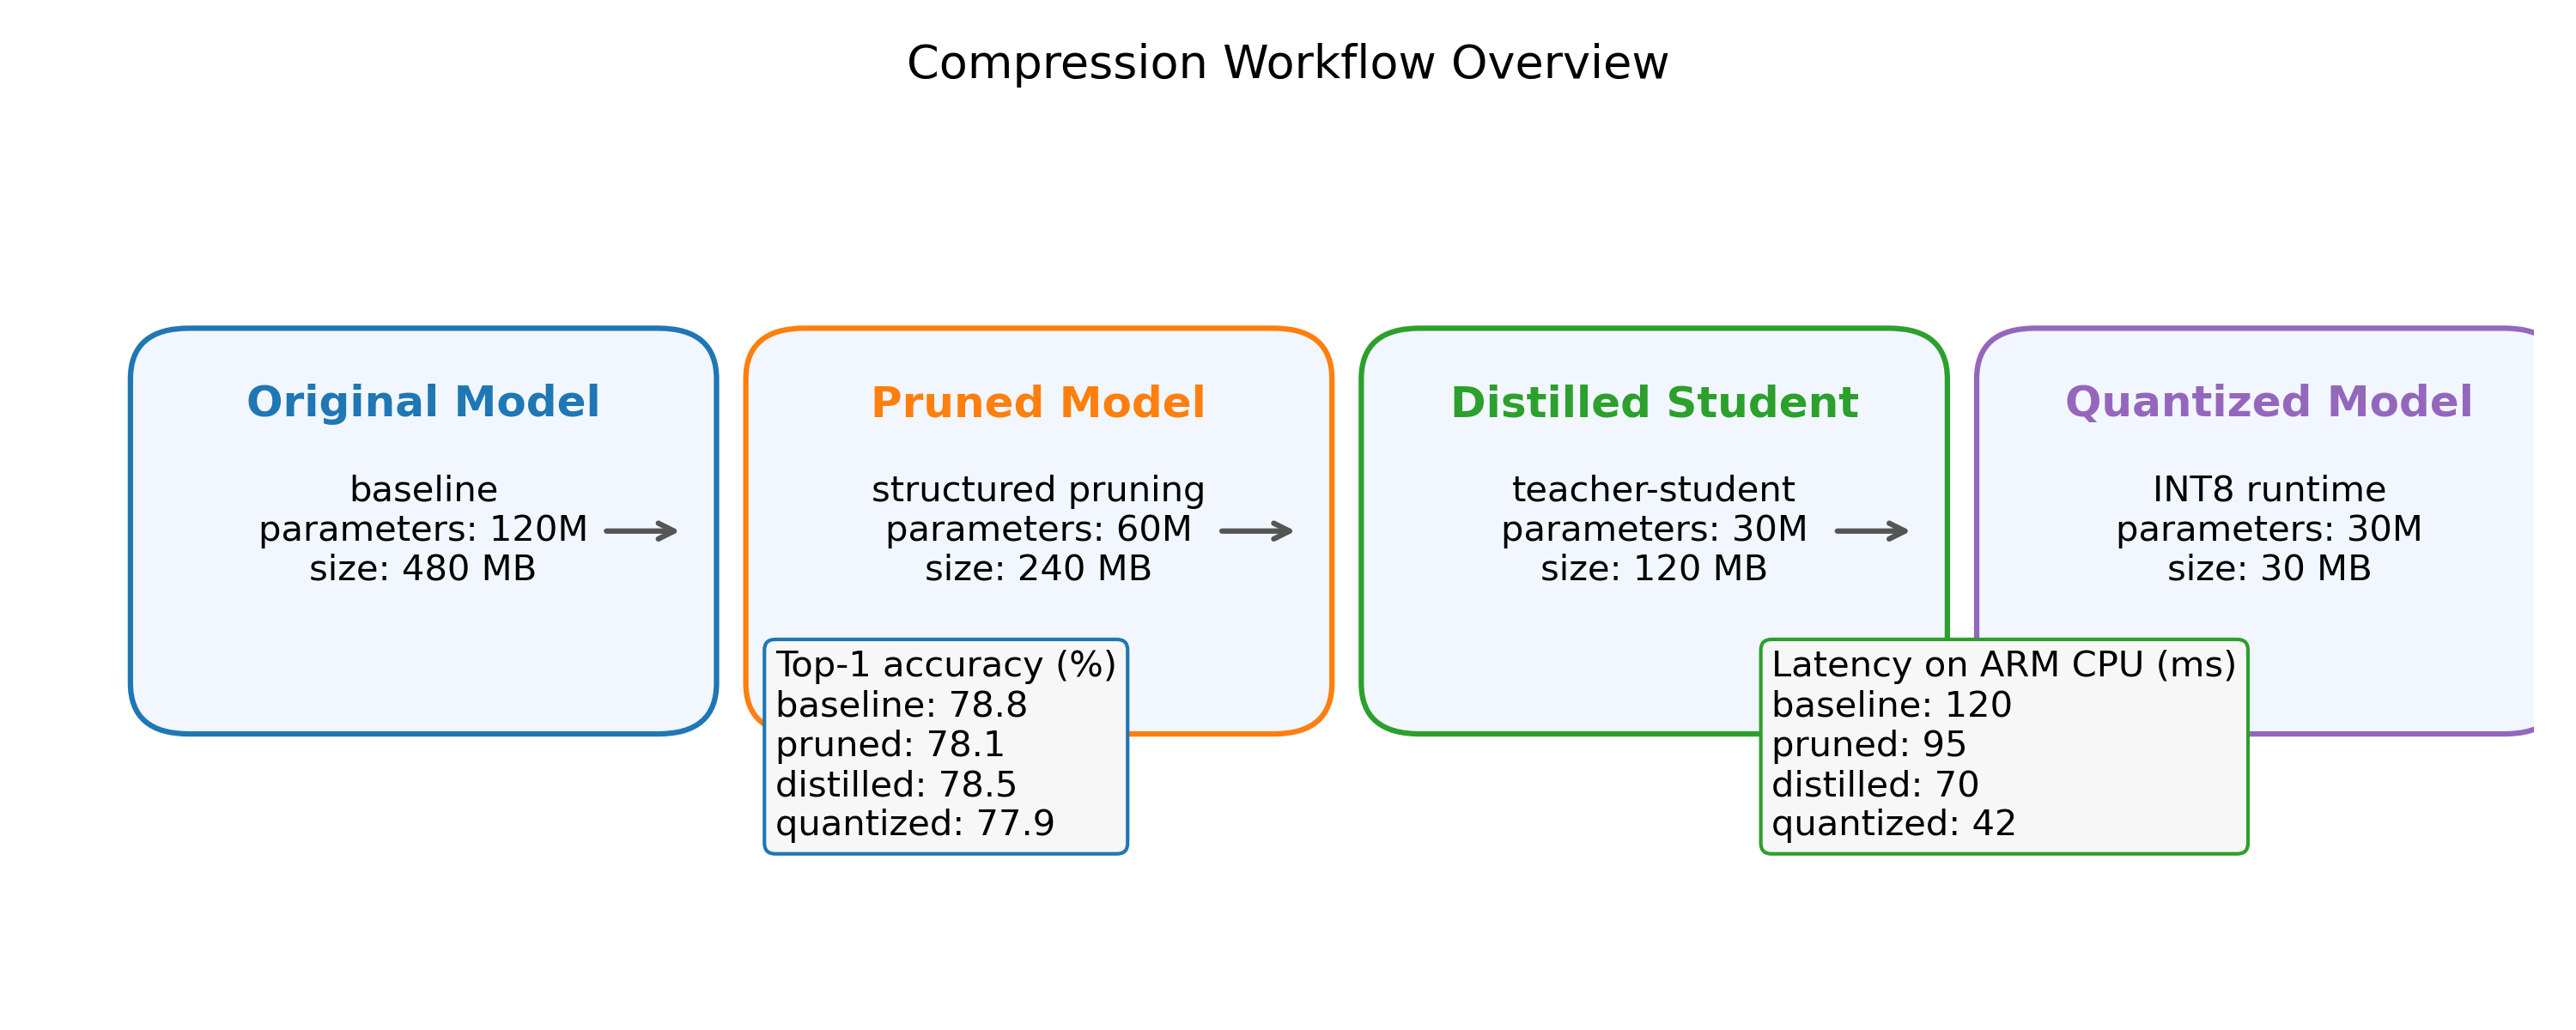
\includegraphics[width=0.9\textwidth]{compression_overview.png}
  \caption{Comparison of pruning, distillation, and quantization pipelines. The bottom row shows accuracy vs. model size trade-offs.}
  \label{fig:compression_overview}
\end{figure}
\FloatBarrier

\section{Deployment to Mobile and Edge (TensorRT, ONNX, TFLite)}
Edge deployment requires toolchains that convert trained models into device-specific runtimes. Figure~\ref{fig:deployment_toolchain} summarizes the major ecosystems.

\subsection{ONNX as an Interchange Format}
The Open Neural Network Exchange (ONNX) defines an intermediate representation (IR) with operator sets (opsets). Exporting from PyTorch or TensorFlow yields a portable graph:
\begin{equation}
  \text{Graph} = (\mathcal{V}, \mathcal{E}, \mathcal{O}),
\end{equation}
where $\mathcal{V}$ are tensors, $\mathcal{E}$ edges, and $\mathcal{O}$ operator nodes. Version alignment between exporter and runtime is critical. Shape inference and constant folding reduce redundancy before deployment.

\subsection{TensorRT Optimization}
TensorRT compiles ONNX graphs into CUDA kernels. Major passes include layer fusion, precision calibration (FP16/INT8), and kernel auto-tuning. The optimization profile specifies input ranges for dynamic shapes. Execution providers (TensorRT EP) integrate into ONNX Runtime to fall back to CPU/GPU operators when unsupported.

\subsection{TensorFlow Lite (TFLite)}
TFLite converts TensorFlow SavedModels into a flatbuffer format with selective operator kernels for mobile CPUs, GPUs, and NPUs. Quantization-aware training can export INT8 kernels compatible with Edge TPU. Delegate mechanisms (e.g., NNAPI, Core ML) offload computation to vendor accelerators.

\subsection{Deployment Checklist}
\begin{itemize}
  \item Validate numerical parity between source framework and exported model via golden tests.
  \item Profiles memory usage and latency under realistic batch sizes and sequence lengths.
  \item Integrate fallback paths: e.g., if TensorRT fails to build an engine, fall back to ONNX Runtime GPU.
  \item Monitor operator coverage; custom ops require plugin development or graph rewriting.
\end{itemize}
The following script demonstrates exporting a PyTorch model to ONNX and building a TensorRT engine using the Python API:

\begin{lstlisting}[language=Python, caption={PyTorch to ONNX export and TensorRT engine building.}]
import torch
import onnx
import tensorrt as trt

model = build_model().eval().cuda()
dummy = torch.randn(1, 3, 224, 224, device="cuda")
torch.onnx.export(model, dummy, "model.onnx",
                  input_names=["input"], output_names=["logits"],
                  opset_version=17, do_constant_folding=True,
                  dynamic_axes={"input": {0: "batch"}, "logits": {0: "batch"}})

onnx_model = onnx.load("model.onnx")
onnx.checker.check_model(onnx_model)

logger = trt.Logger(trt.Logger.INFO)
builder = trt.Builder(logger)
network = builder.create_network(1 << int(trt.NetworkDefinitionCreationFlag.EXPLICIT_BATCH))
parser = trt.OnnxParser(network, logger)
with open("model.onnx", "rb") as f:
    parser.parse(f.read())

config = builder.create_builder_config()
config.set_memory_pool_limit(trt.MemoryPoolType.WORKSPACE, 1 << 30)
if builder.platform_has_fast_int8:
    config.set_flag(trt.BuilderFlag.INT8)
    config.int8_calibrator = gather_calibration_data()

engine = builder.build_engine(network, config)
with open("model.plan", "wb") as f:
    f.write(engine.serialize())
\end{lstlisting}

\begin{figure}[H]
  \centering
  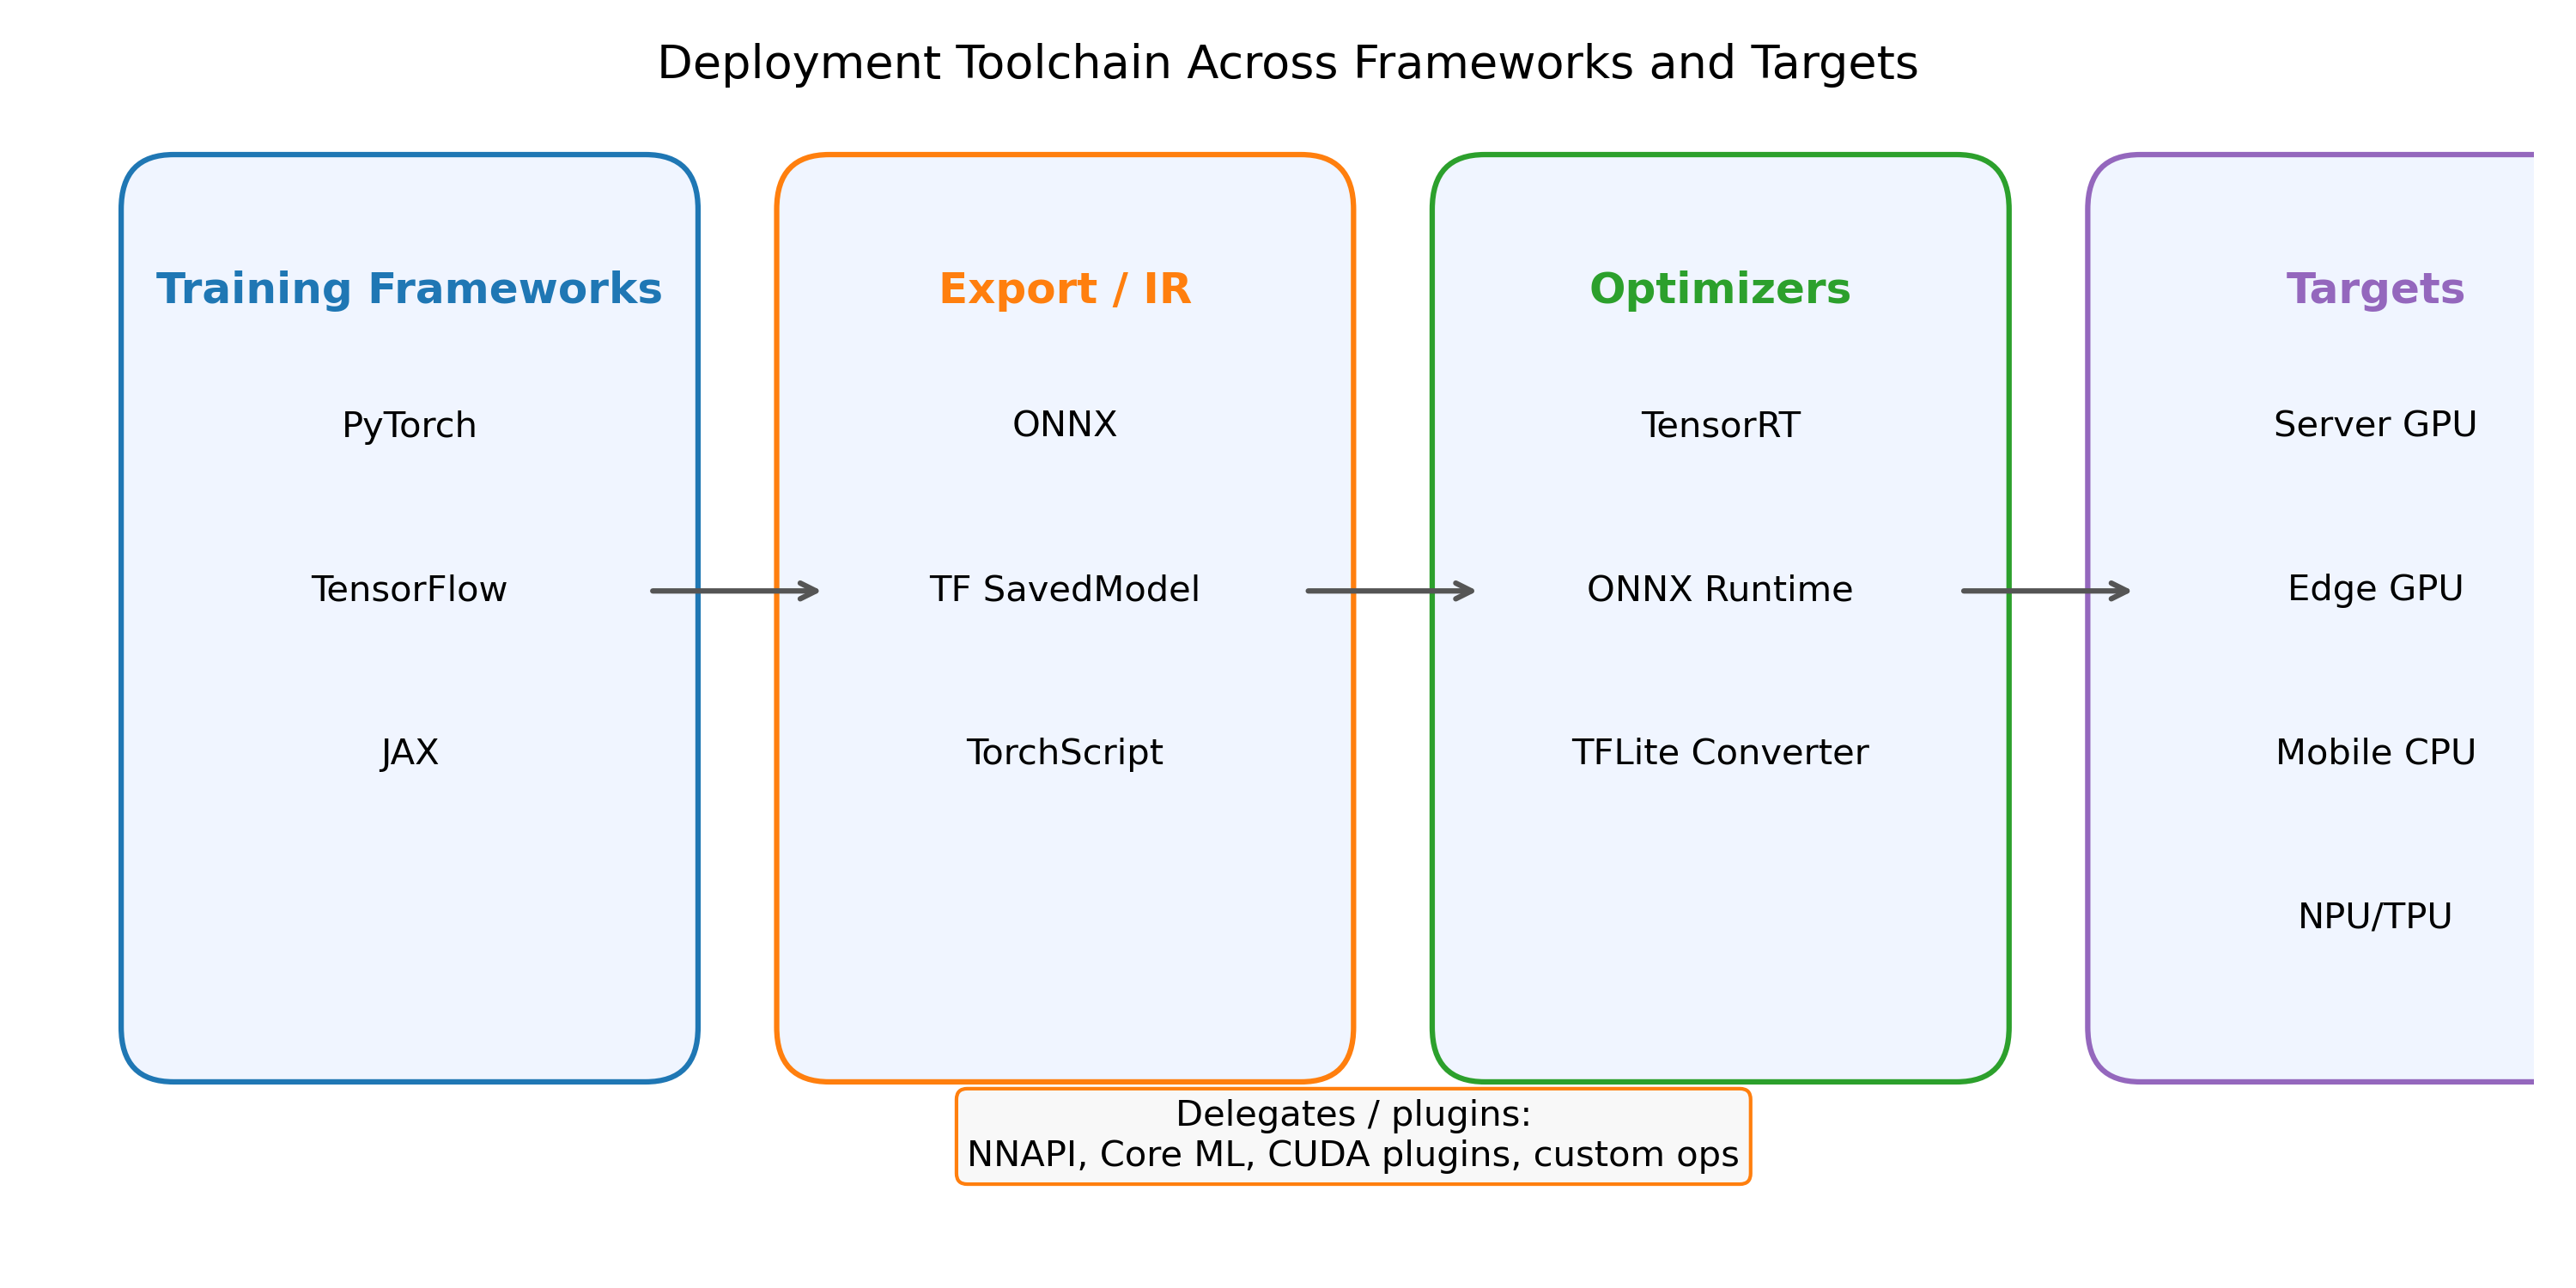
\includegraphics[width=0.9\textwidth]{deployment_toolchain.png}
  \caption{Deployment toolchains across ONNX, TensorRT, and TensorFlow Lite. Optional delegates target vendor accelerators.}
  \label{fig:deployment_toolchain}
\end{figure}
\FloatBarrier

\section{Inference Acceleration}
Inference optimization targets latency, throughput, and energy efficiency. Figure~\ref{fig:latency_breakdown} shows a latency decomposition, while Figure~\ref{fig:accelerated_inference_strategies} outlines common acceleration strategies.

\subsection{Kernel and Graph Optimizations}
Operator fusion merges sequences like Conv-BN-ReLU into a single kernel, reducing memory traffic. Graph compilers (TVM, XLA, TorchInductor) apply loop tiling, vectorization, and layout transformations. The latency $L$ can be approximated as
\begin{equation}
  L = \sum_{i=1}^{N} \left(\frac{C_i}{\mathrm{FLOP/s}} + \frac{M_i}{\mathrm{BW}}\right),
\end{equation}
where $C_i$ is compute cost and $M_i$ memory traffic. Tuning seeks to minimize both components via scheduling.

\subsection{Batching and Dynamic Serving}
Batching amortizes overhead across requests. For online systems with arrival rate $\lambda$ and service rate $\mu$, queueing delay is governed by the Erlang C formula. Dynamic batching (Triton Inference Server) accumulates requests up to latency budgets. For autoregressive models, speculative decoding and scheduling partial beams reduce token latency.

\subsection{Hardware Acceleration}
Specialized accelerators (Edge TPU, NVIDIA Tensor Cores) offer mixed-precision support. Memory-bound models benefit from high-bandwidth memory (HBM) and sparsity-aware hardware. For edge deployments, CPU vector engines (NEON, AVX512) are leveraged via libraries like XNNPACK and oneDNN.

\subsection{Monitoring and A/B Testing}
Production systems require continuous measurement of latency percentiles (P50/P95/P99), throughput, and energy consumption. Canary releases test optimized models on a subset of traffic to ensure stability. Rollback procedures and feature flags guard against degraded user experience.

\begin{lstlisting}[language=Python, caption={Triton Inference Server dynamic batching configuration (YAML).}]
name: "resnet_triton"
platform: "tensorrt_plan"
max_batch_size: 32
input [
  { name: "input", data_type: TYPE_FP16, dims: [3, 224, 224] }
]
output [
  { name: "logits", data_type: TYPE_FP16, dims: [1000] }
]
dynamic_batching {
  preferred_batch_size: [4, 8, 16, 32]
  max_queue_delay_microseconds: 2000
}
instance_group [
  { kind: KIND_GPU, count: 2, gpus: [0, 1] }
]
\end{lstlisting}

\begin{figure}[H]
  \centering
  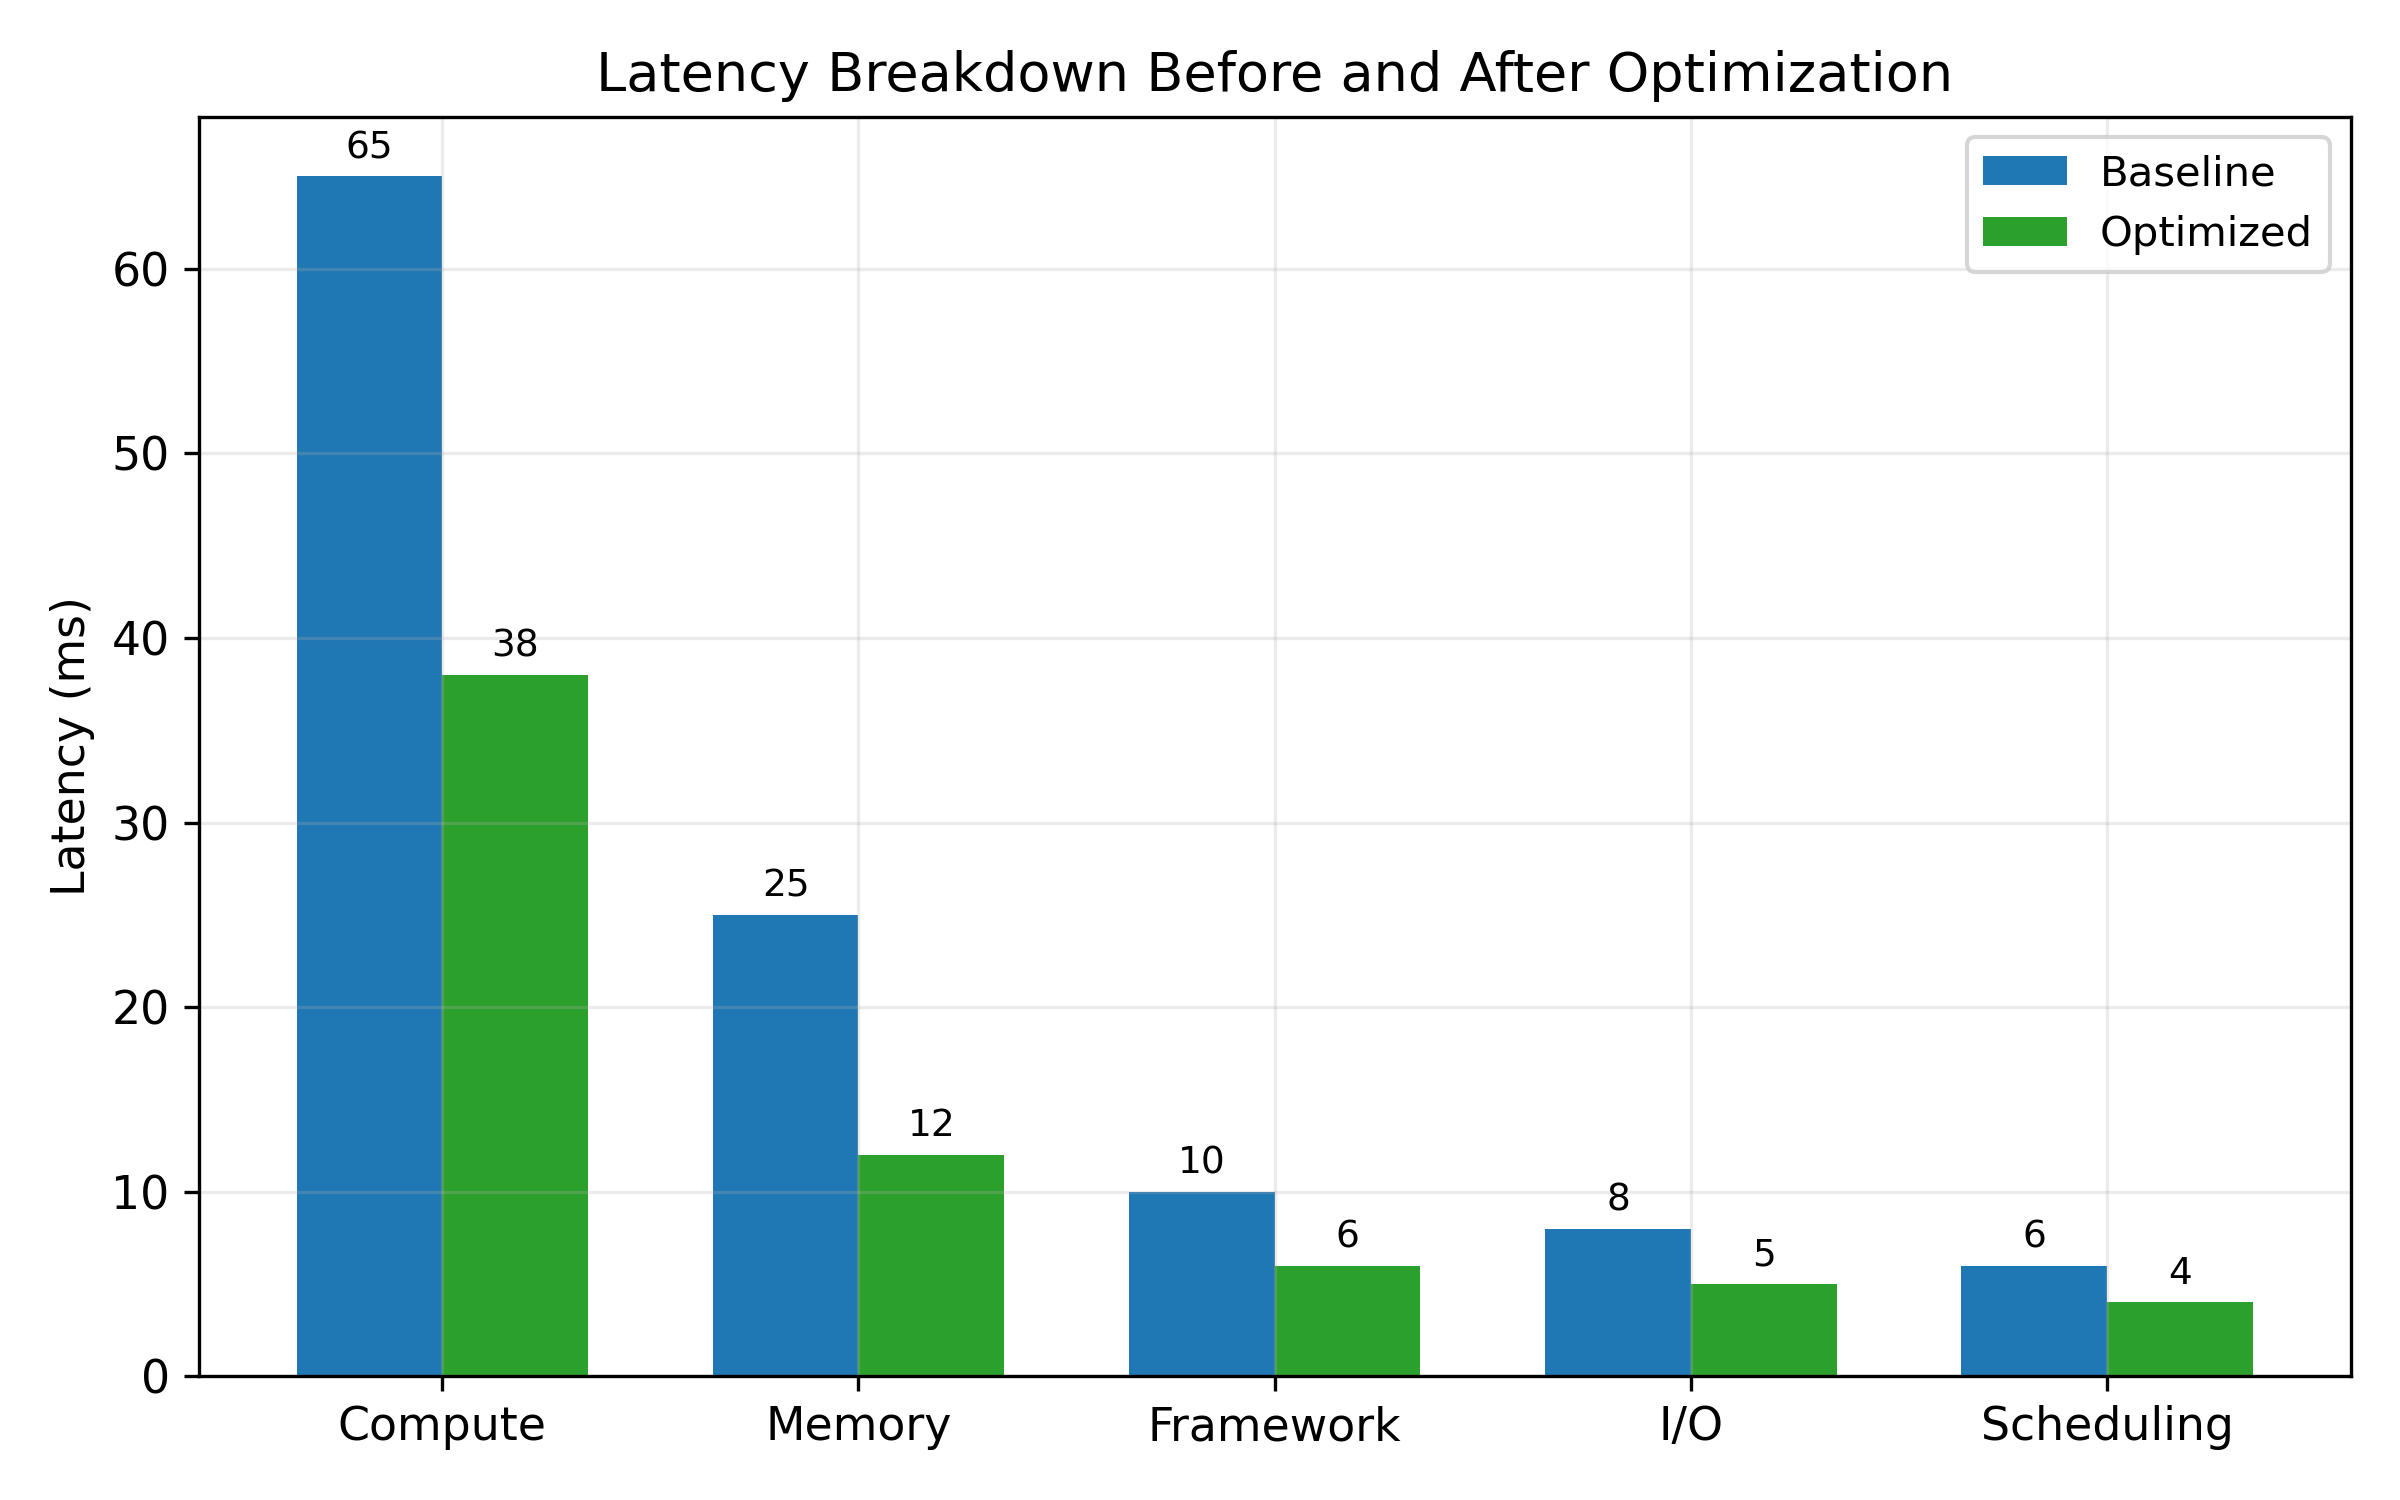
\includegraphics[width=0.85\textwidth]{latency_breakdown.png}
  \caption{Latency breakdown across compute, memory, and I/O components. Profiling highlights the dominant bottleneck.}
  \label{fig:latency_breakdown}
\end{figure}

\begin{figure}[H]
  \centering
  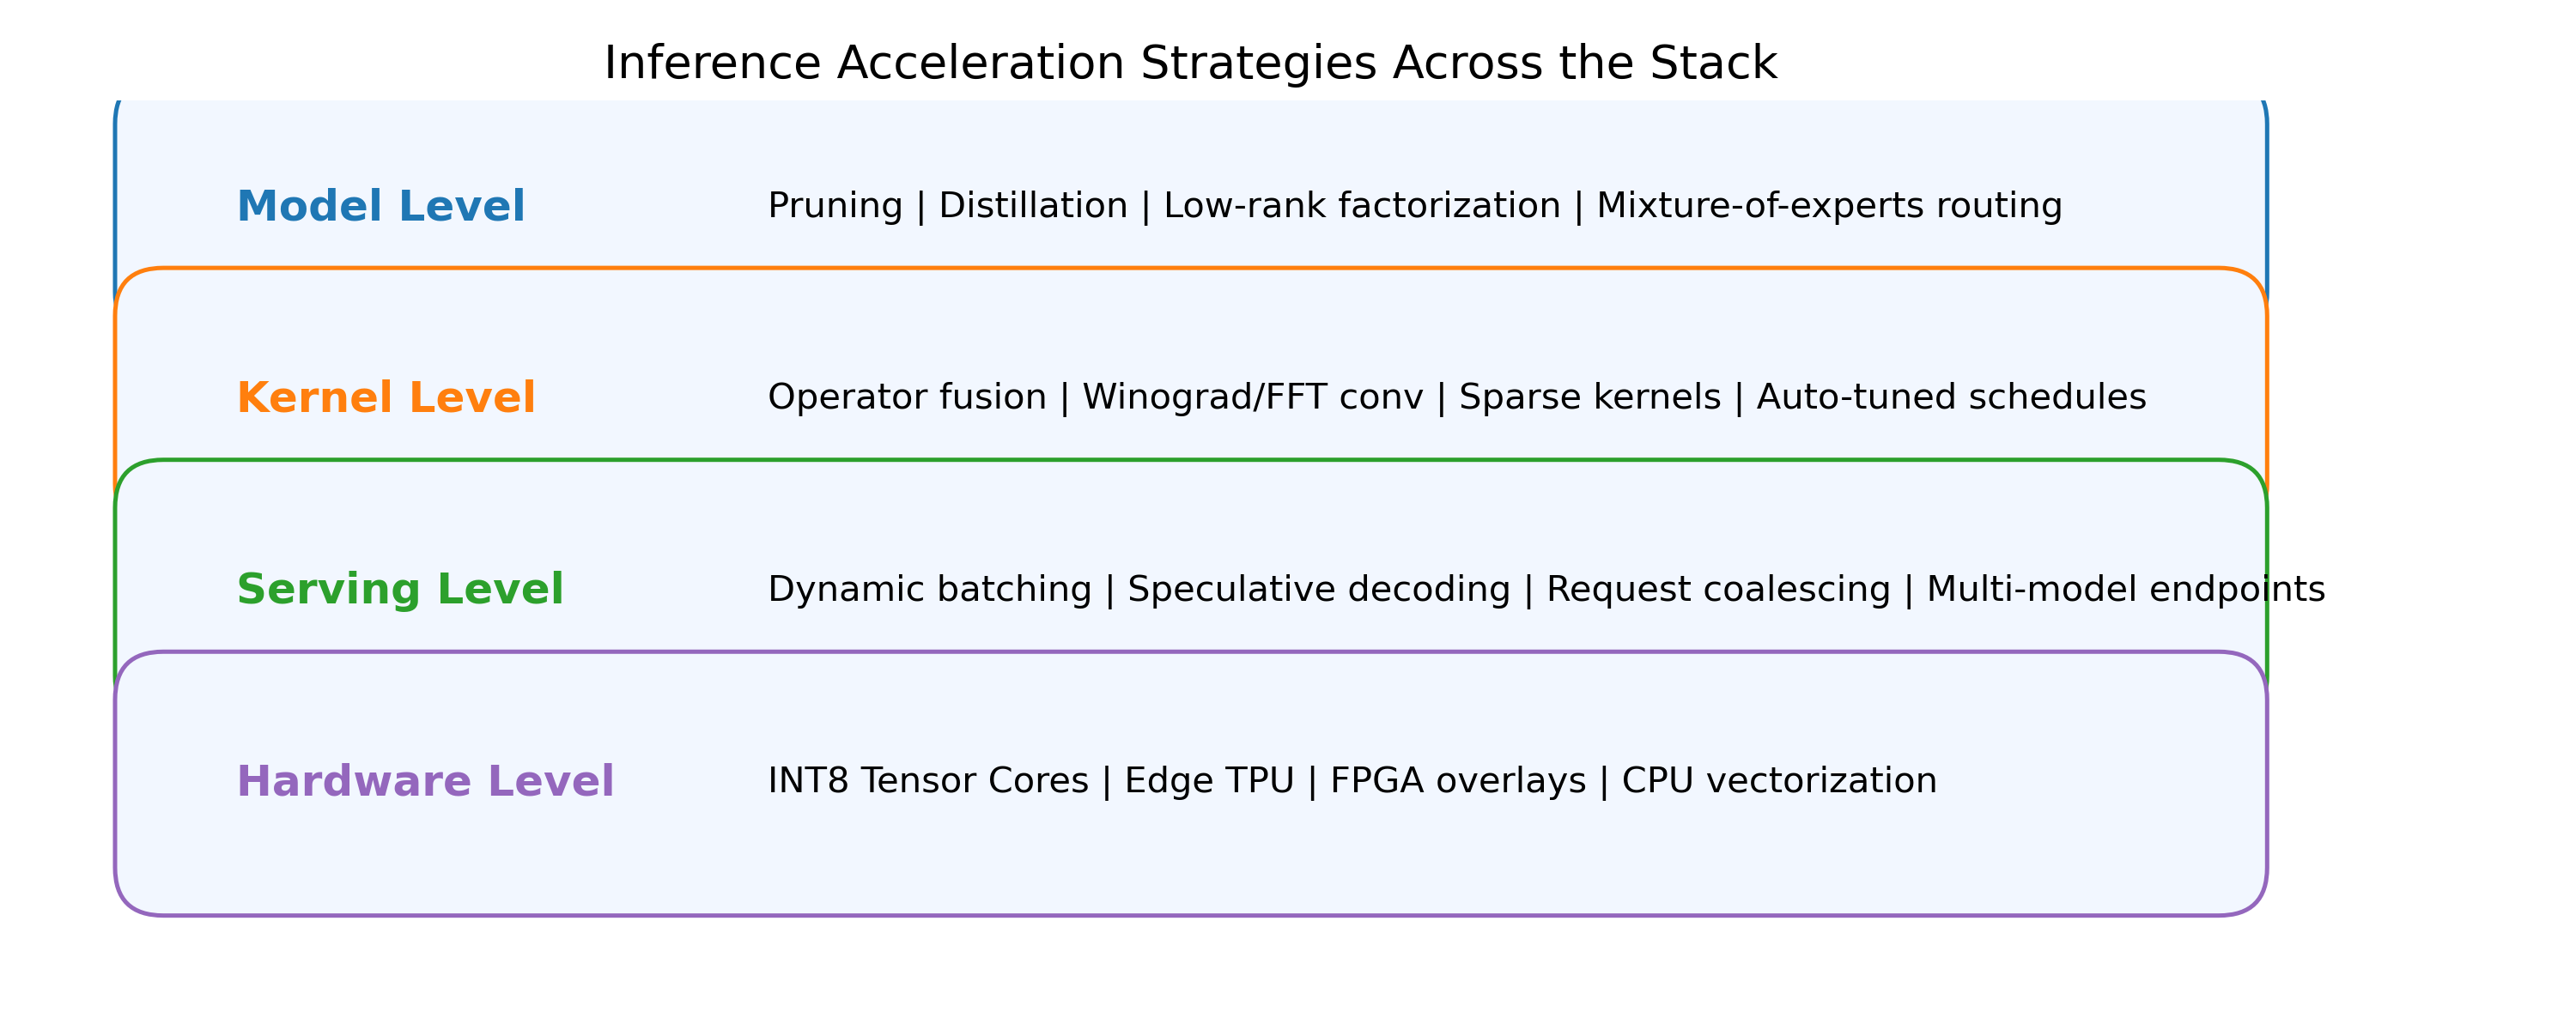
\includegraphics[width=0.9\textwidth]{accelerated_inference_strategies.png}
  \caption{Inference acceleration strategies spanning model, kernel, serving, and hardware layers.}
  \label{fig:accelerated_inference_strategies}
\end{figure}
\FloatBarrier

\section*{Further Reading}
\begin{itemize}
  \item Song Han et al. ``Learning both Weights and Connections for Efficient Neural Networks.'' NIPS 2015.
  \item Geoffrey Hinton et al. ``Distilling the Knowledge in a Neural Network.'' NIPS 2015 Workshop.
  \item Jacob et al. ``Quantization and Training of Neural Networks for Efficient Integer-Arithmetic-Only Inference.'' CVPR 2018.
  \item NVIDIA. ``TensorRT Developer Guide.'' 2023.
  \item Jared Casper et al. ``Amazon SageMaker Inference Recommender.'' 2022.
\end{itemize}

\end{document}
